\documentclass{article}
\usepackage[english]{babel}
\usepackage{ragged2e}
\usepackage{blindtext}
\usepackage{natbib}
\usepackage{graphicx}
\usepackage{biblatex}
\usepackage{amsmath}
\usepackage{algorithm}
\usepackage{algpseudocode}

\addbibresource{references.bib}

\title{Sense of direction in \textit{tori}}
\author{Szymon Szulc}
\date{January 2024}

\begin{document}
\maketitle

\section{Topological structure}
Informally \textit{torus} is a two-dimensional (wrap-around) array of $n$ processors. It is a regular graph. Each processor has exactly 4 neighbours.
\textit{Torus} of dimensions $a \times b $ has $n = ab$ processors $v_i_,_j(0 <= i <= a - 1, 0 <= j <= b - 1)$. Each node $v_i_,_j$ is connected by a bidirectional link with $v_i_,_j_+_1$, $v_i_,_j_-_1$, $v_i_+_1,_j$, 
$v_i_-_1_,_j$, where all
the operations on the first index are $\textit{modulo } a$, while those on the second index are
$\textit{modulo } b$ (Figure 1). For the rest of sections, I will assume that, \textit{torus} is a square \mbox{$a=b=\sqrt{n}$}.

\begin{figure}[h!]
\centering
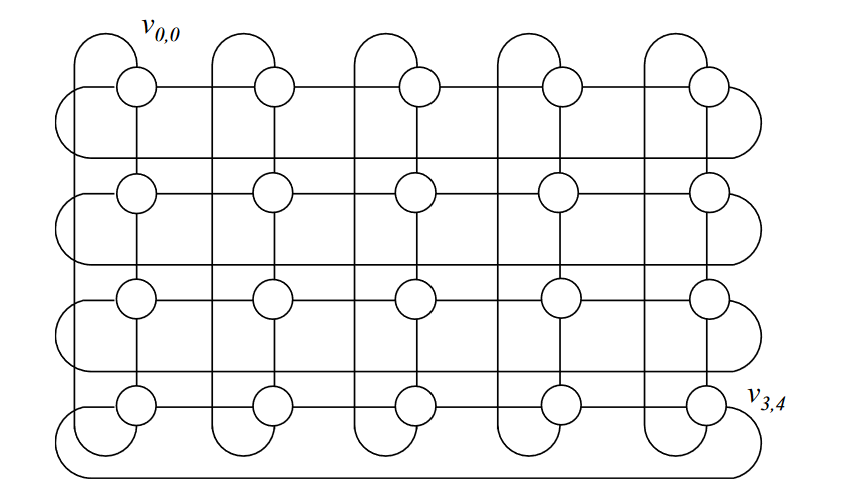
\includegraphics{torus.png}
\caption{Torus $4 \times 5$ \cite{mans}}
\label{fig:torus}
\end{figure}

\newpage

\section{Sense of direction in \textit{tori}}
Imagine you are looking at the network from a bird's-eye view. Each edge has a label from the set $\{north, south, east, west\}$ assigned in the
natural globally consistent way (Figure 2). Having such a labeling, it is trivial to check if 2 paths lead to the same processor. The lack of sense of direction is known to increase the message complexity of the election problem. For example in a \textit{torus} we can choose leader in $\Theta(n)$, instead of $\Theta(n\log{}n)$ \cite{mans}, when nodes have the sense of direction.

\begin{figure}[h!]
\centering
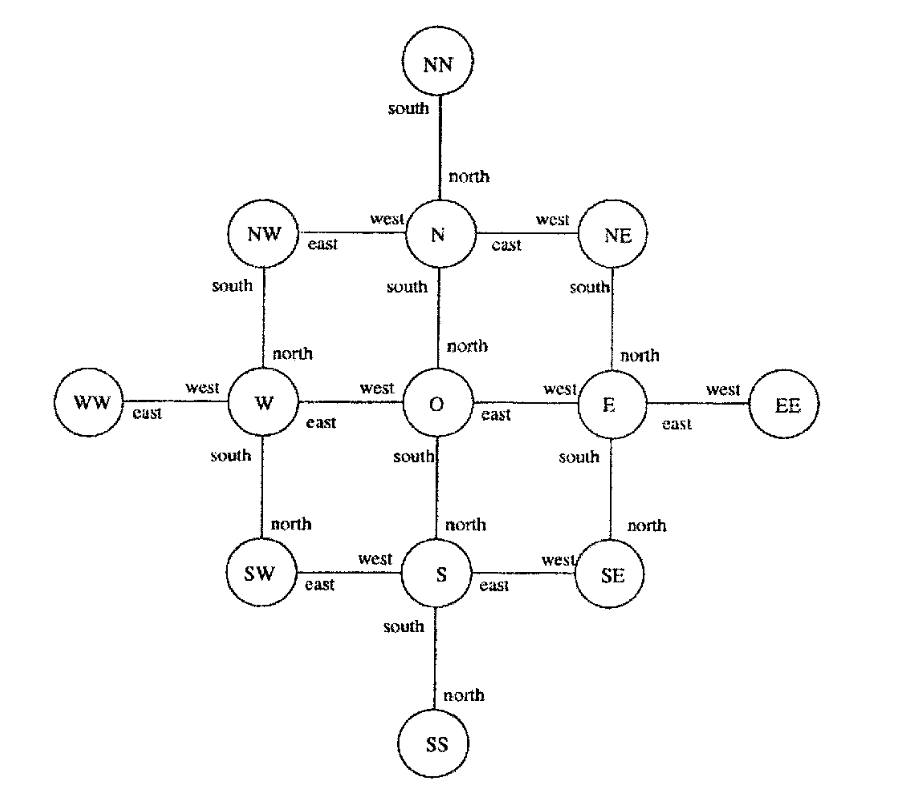
\includegraphics[scale=0.9]{labels.png}
\caption{Labels of the edges \cite{mans}}
\label{fig:torus}
\end{figure}

\newpage

\section{Outline of leader election algorithm}  
The main idea behind Peterson’s algorithm for square bidirectional \textit{tori} is marking territory. In each stage, each processor tries to mark off the boundary of a square distance $d$ on a side ($d=\alpha^i$ for some constant $\alpha$). If node closes boundary, it survives to the next stage. If node's message encounters territory with lower \textit{id}. it does not survive, because boundary with lower \textit{id} purges its message. Peterson shows, that $\alpha=1.1795$ to obtain $\Theta(n)$. Peterson also suggested, that “the algorithm only
needs to mark off a square; the orientation of the square
is irrelevant.”\cite{peterson}

\section{Getting a local sense of direction}

\begin{subsection}{Main idea}
We only need the processor to pass message in straight line or make appropriate turn. Is relatively easy to obtain. Each processor has to know the identity and the position of each processor at distance 2.   
\end{subsection}

\begin{subsection}{Algorithm}
In a nutshell, each processor sends its identity to each of its neighbors, which forwards it to its three remaining neighbors.

\begin{algorithm} 
\caption{Bernard Mans' algorithm for local sense of direction in \textit{tori}}
\begin{algorithmic}
\State $\forall \ \text{link} \ r \ \text{initialize} \ H1_r:=\emptyset,\ H2_r:=\emptyset$
\State $\forall \ \text{link} \ k \ \text{send ONE(myId) on arc k}$
\\
\Repeat
    \State \Call{Receive}{}
\Until received 16 messages
\\
\Procedure{Receive}{$message(type, \ id, \ link)$}
    \If{$type = ONE$}
        \State $H1_\text{link}:=\{id\}$
        \State $\forall \ \text{link} \ k \neq link  \ \text{send TWO(id) on arc k}$
    \EndIf
    \If{$type = TWO$}
        \State $H2_\text{link}:=H2_\text{link} \cup \{id\}$    
    \EndIf
\EndProcedure
\end{algorithmic}
\end{algorithm}

\newpage

After execution of this algorithm each node knows:
\begin{itemize}
    \item its immediate neighbours
    \item links must be used to reach them
    \item nodes at distance 2
\end{itemize}
The amount of information is enough to pass messages straight and make appropriate turns. If $H2_i \cap H2_j = \emptyset$, then links $i$ and $j$ are parallel, else they are perpendicular. (this statement is $true$ for $\sqrt{n} > 4$) 

\end{subsection}

\begin{subsection}{Handrail}
We already know how to pass messages in straight lines. But how to make appropriate turns? Initiator node chooses 2 perpendicular links. Using one of them, sends message containing other link immediate neighbour - $handrail$. When node receives such message, it exactly knows, which link  ($k$) to choose to make appropriate turn
$(H2_\text{linkFrom} \cap H2_k = handrail)$.  
\end{subsection}

\begin{subsection}{Complexity}
Each processor sent 4 messages to its immediate neighbors and passed \mbox{$4 \times 3$ messages}, that is $16n$ messages overall. So this algorithm has message complexity $\Theta(n)$. 
\end{subsection}

\printbibliography
\end{document}
